\documentclass[10pt]{beamer}
\usetheme{metropolis}
\usepackage{booktabs}
\usepackage{tabularx}
\usepackage{calc}
\usepackage{tikz}
\usepackage[sfdefault]{FiraSans}
\usepackage[scaled]{FiraMono}
\usetikzlibrary{shapes.geometric, arrows, positioning, decorations.pathreplacing}

% Setup for faculty images
\newlength{\imageheight}
\setlength{\imageheight}{3.5cm}

% Define CSUF brand colors
\definecolor{titanblue}{HTML}{00244E}
\definecolor{mediumblue}{HTML}{0F3F8C}
\definecolor{skyblue}{HTML}{EBFBFF}
\definecolor{titanorange}{HTML}{FF7900}
\definecolor{titangray}{HTML}{F5F5F5}
\definecolor{titantext}{HTML}{222222}

% Customize metropolis theme colors
\setbeamercolor{normal text}{fg=titantext, bg=white}
\setbeamercolor{alerted text}{fg=titanorange}
\setbeamercolor{example text}{fg=mediumblue}

% Title page colors
\setbeamercolor{title}{fg=titanblue, bg=white}
\setbeamercolor{subtitle}{fg=mediumblue, bg=white}
\setbeamercolor{institute}{fg=titanorange, bg=white}
\setbeamercolor{date}{fg=titanblue, bg=white}

% Frame title colors
\setbeamercolor{frametitle}{fg=white, bg=titanblue}
\setbeamercolor{framesubtitle}{fg=mediumblue, bg=white}

% Block environment colors
\setbeamercolor{block title}{fg=white, bg=titanblue}
\setbeamercolor{block body}{fg=titantext, bg=skyblue!10}

% Item colors
\setbeamercolor{itemize item}{fg=titanorange}
\setbeamercolor{itemize subitem}{fg=mediumblue}
\setbeamercolor{itemize subsubitem}{fg=titanblue}

% Footer and header colors
\setbeamercolor{footer}{fg=titantext}
\setbeamercolor{header}{fg=titanblue}

% Custom TikZ embellishments for POSC 315 Beamer slides
\usepackage{tikz}
\usetikzlibrary{shadows,arrows.meta,positioning,shapes.multipart}

% Boxed text for emphasis
\newcommand{\tikzbox}[2][]{
  \begin{tikzpicture}
    \node[draw=mediumblue, fill=skyblue!20, thick, rounded corners, inner sep=10pt, text width=0.9\textwidth,#1] {#2};
  \end{tikzpicture}
}

% Horizontal divider with arrow
\newcommand{\tikzdivider}{
  \begin{center}
  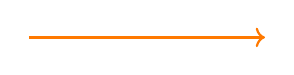
\begin{tikzpicture}
    \draw[->, thick, titanorange] (0,0) -- (3,0);
  \end{tikzpicture}
  \end{center}
}

% Highlighted comparison row (e.g., for causation slides)
\newcommand{\relationrow}[2]{
  \begin{tikzpicture}
    \node[draw=none, fill=titangray!50, rounded corners, text width=0.9\textwidth, inner sep=8pt] {
      \textbf{#1} \hfill #2
    };
  \end{tikzpicture}
}

% Framed callout block
\newcommand{\callout}[1]{
  \begin{tikzpicture}
    \node[draw=titanorange, fill=white, thick, rounded corners, inner sep=10pt, text width=0.9\textwidth] {
      \textit{#1}
    };
  \end{tikzpicture}
}

% Customize fonts
\setbeamerfont{title}{size=\Large, series=\bfseries}
\setbeamerfont{frametitle}{size=\large, series=\bfseries}

% Simple title page template
\defbeamertemplate*{title page}{customized}[1][]
{
\vspace{1cm}
 {\usebeamerfont{title}\usebeamercolor[fg]{title}\inserttitle\par}
\vspace{0.5cm}
 {\usebeamerfont{subtitle}\usebeamercolor[fg]{subtitle}\insertsubtitle\par}
\vspace{0.5cm}
 {\usebeamerfont{date}\usebeamercolor[fg]{date}\insertdate\par}
\vfill
 {\insertinstitute\par}
}

% Add progress bar
\makeatletter
\setbeamertemplate{headline}{%
\begin{beamercolorbox}[wd=\paperwidth,ht=0.4cm,dp=0cm]{titanblue}%
\begin{tikzpicture}
\pgfmathsetmacro{\progress}{\insertframenumber/\inserttotalframenumber}
\fill[titanorange] (0,0) rectangle (\progress*\paperwidth,0.4cm);
\end{tikzpicture}%
\end{beamercolorbox}%
}
\makeatother

\begin{document}

\title{Understanding Politics and Public Policy}
\subtitle{Foundations and Core Concepts\\POSC 315: Introduction to Public Policy\\Lecture 9-2: Policy Analysis Part 2}
\date{David P. Adams, Ph.D.}
\institute{California State University, Fullerton}

\maketitle


\begin{frame}{Analyst Roles}

\begin{block}{}
    \textbf{Objective Technician:}
    \begin{itemize}
        \item Independent, neutral
        \item Predicts outcomes, avoids advocacy
    \end{itemize}

    \textbf{Client's Advocate:}
    \begin{itemize}
        \item Supports client's position
        \item Strategic use of evidence
    \end{itemize}

    \textbf{Issue Advocate:}
    \begin{itemize}
        \item Uses analysis to push societal goals
        \item Accepts role as political actor
    \end{itemize}
\end{block}


\end{frame}


\begin{frame}{Bardach’s Eightfold Path}

% \begin{tikzpicture}[node distance=1.2cm, every node/.style={rectangle, draw=titanblue, fill=skyblue!20, rounded corners, text width=0.9\textwidth, align=left, font=\small}]
% \node (step1) {\textbf{1. Define the problem}};
% \node (step2) [below=of step1] {\textbf{2. Assemble evidence}};
% \node (step3) [below=of step2] {\textbf{3. Construct alternatives}};
% \node (step4) [below=of step3] {\textbf{4. Select criteria}};
% \node (step5) [below=of step4] {\textbf{5. Project outcomes}};
% \node (step6) [below=of step5] {\textbf{6. Confront trade-offs}};
% \node (step7) [below=of step6] {\textbf{7. Decide}};
% \node (step8) [below=of step7] {\textbf{8. Tell your story}};
% \end{tikzpicture}

\begin{itemize}
  \item Define the problem
  \item Assemble evidence
  \item Construct alternatives
  \item Select criteria
  \item Project outcomes
  \item Confront trade-offs
  \item Decide
  \item Tell your story
\end{itemize}

\end{frame}


\begin{frame}{Two Logics of Policy}

\begin{block}{}
    \textbf{Economic Rationality (Analysts):}
    \begin{itemize}
        \item Transparent assumptions
        \item Compare alternatives systematically
    \end{itemize}

    \textbf{Political Rationality (Policymakers):}
    \begin{itemize}
        \item Incentive-driven
        \item Selectively emphasize data
        \item Consider feasibility
    \end{itemize}
\end{block}

\end{frame}


\begin{frame}{Bridging the Logics}

\begin{block}{}
    \begin{itemize}
        \item Both views are valid
        \item Policy isn't purely rational — or irrational
        \item Political realities matter
        \item Good analysis blends rigor with context
    \end{itemize}
\end{block}

\end{frame}


\begin{frame}{Why Politics Matters}

\begin{block}{}
    \begin{itemize}
        \item Explains “irrational” outcomes
        \item Informs institutional design
        \item Prepares analysts to act strategically
        \item Values and preferences matter in policy
    \end{itemize}
\end{block}

\end{frame}


\begin{frame}{Evolution of the Profession}

\begin{block}{}
    \begin{itemize}
        \item More diverse, specialized roles
        \item Analysts are not neutral technicians
        \item Engagement and inclusion are emphasized
        \item Technical skills still essential, but not enough
    \end{itemize}
\end{block}

\end{frame}


\begin{frame}{Let’s Try It: Wild Horse Case}

\begin{block}{}
    \textbf{The Problem:} Wild horse overpopulation on public lands

    \textbf{Goals:} Sustainability, ecological health, humane treatment

    \textbf{Alternatives:}
    \begin{itemize}
        \item Adoption
        \item Fertility control
        \item Habitat expansion
    \end{itemize}

    \textbf{Criteria:} Cost, effectiveness, feasibility, animal welfare
\end{block}

\end{frame}


\begin{frame}{Video: Horse Rich and Dirt Poor}

\callout{Watch: \url{https://www.youtube.com/embed/q6h242vy_q8}}

\end{frame}


\begin{frame}{Reflections on the Case}

\begin{block}{}
    \begin{itemize}
        \item Balance values: ecology, economy, ethics
        \item Mix of strategies may be required
        \item Must account for stakeholder perspectives
        \item Evaluation + adaptation are key to success
    \end{itemize}
\end{block}

\end{frame}


\begin{frame}{That's All for Today}

\centering
\callout{Questions? Comments?}

\end{frame}

\end{document}
